\chapter{Radicalen, carbenen en omleggingen}\label{ch:b3:radicals-carbenes}

De pyrethrummargriet verdedigt zich met esters van chrysanthemumzuur,
moleculen die rond een ring van drie koolstofatomen gebouwd zijn; hun
synthetische verwanten behoren tot de meest gebruikte insecticiden in
huis. Chemici sluiten zulke ringen in één stap door een \omterm{def:b3:organometallic-bonding:carbene}{carbeen} aan een
dubbele binding te adderen: een koolstofatoom met maar zes elektronen
eromheen, waarvan er twee niet gedeeld zijn. Dit hoofdstuk behandelt
reactieve intermediairen die de delen van jaar~1 en jaar~2 alleen
terloops ontmoetten (radicalen in de synthese, \omterm{def:b3:organometallic-bonding:carbene}{carbenen} en nitrenen) en
de omleggingen waarbij een groep naar een elektronenarm koolstof-,
stikstof- of zuurstofatoom verhuist, waaronder twee die uit hetzelfde
keton de monomeren van nylon-6 en van een biologisch afbreekbare
polyester maken.

\begin{recall}
Het deel van jaar~1 voerde radicalen, homolyse en halve pijlen in,
carbokationen en hun omleggingen, nucleofielen en uittredende groepen;
het deel van jaar~2 radicaalketens (initiatie, propagatie, terminatie,
radicaalinitiatoren), peroxyzuren, lactonen, lactamen en imines.
\Cref{ch:b3:complex-kinetics} behandelde de kinetiek van
\omterm{def:b3:complex-kinetics:chain}{kettingreacties},
\cref{ch:b3:organometallic-bonding} \omterm{def:b3:organometallic-bonding:carbene}{carbenen} als liganden,
\cref{ch:b3:many-electron-atoms} singulet- en \omterm{def:b3:many-electron-atoms:singlet-triplet}{triplettoestanden}, en
\cref{ch:b3:rate-theories} het postulaat van Hammond.
\end{recall}

\begin{omfigure}
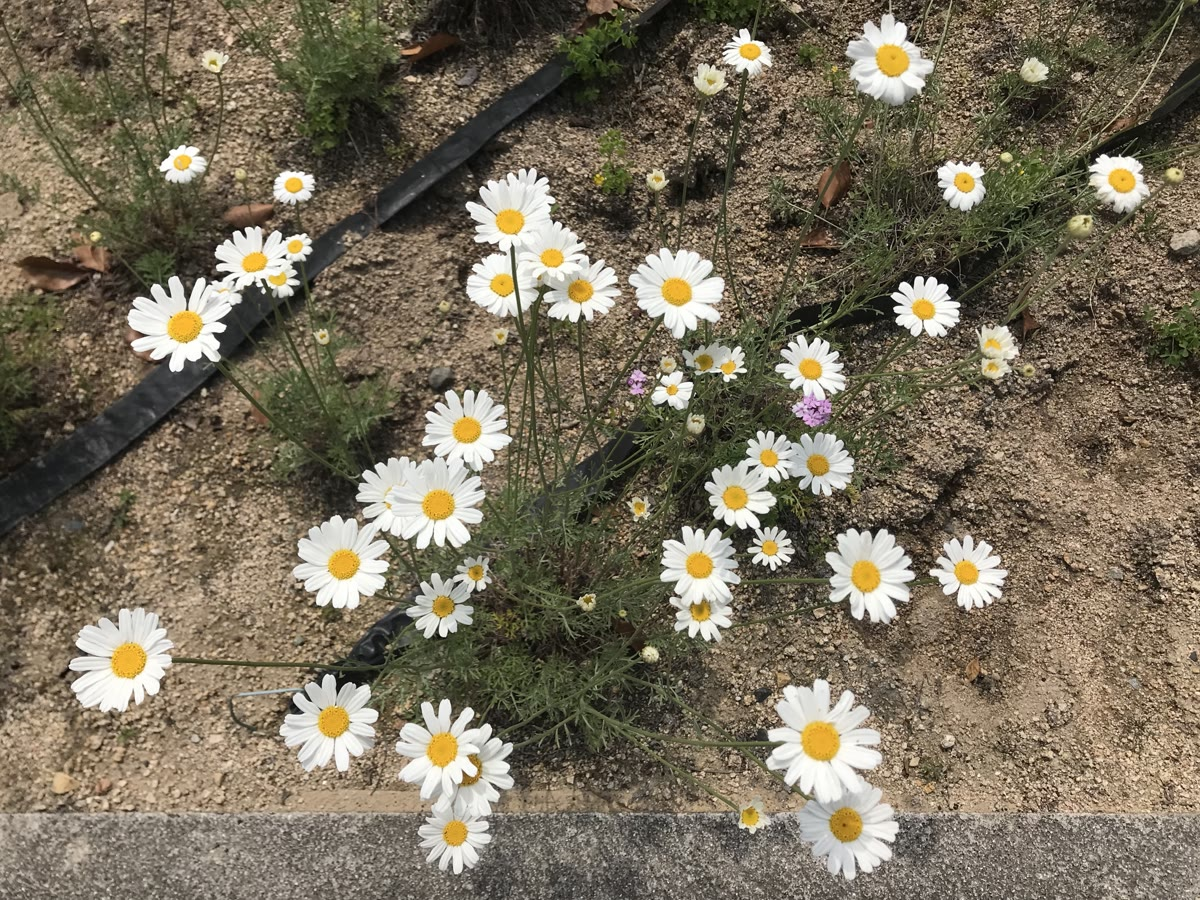
\includegraphics[width=0.48\linewidth]{images/book4/pyrethrum.jpg}

{\small Pyrethrummargrieten. Hun bloemen bevatten de pyrethrinen,
insecticide esters van een cyclopropaancarbonzuur. Foto: Soramimi, CC BY-SA 4.0.}
\end{omfigure}

\section{Radicaalkettingreacties in de synthese}

De stabiliteit van een koolstofradicaal wordt gemeten met de
bindingsdissociatie-enthalpie van de binding C--H die het zou vormen:
hoe zwakker de binding, hoe stabieler het radicaal.

\begin{proposition}[Bindingsdissociatie-enthalpieën]\label{prop:b3:radicals-carbenes:bde}
De bindingsdissociatie-enthalpie van R--H bij \qty{298}{K} volgt uit de
vormingsenthalpieën in de gasfase:
$\mathrm{BDE(R{-}H)} = \Delta_fH^\circ(\mathrm R^\bullet) + \Delta_fH^\circ(\mathrm H^\bullet) - \Delta_fH^\circ(\mathrm{RH})$.
\end{proposition}

\begin{proof}
De homolyse $\mathrm{RH \to R^\bullet + H^\bullet}$ heeft volgens de wet van Hess als reactie-enthalpie de vorming van
de producten min die van de beginstof; die reactie-enthalpie is per
definitie de bindingsdissociatie-enthalpie.
\end{proof}

\begin{omfigure}
% ledger: dfh4:CH3r, dfh4:C2H5r, dfh4:iC3H7r, dfh4:tC4H9r, dfh4:PhCH2r, dfh4:H, dfh:CH4_g, dfh:C2H6_g, dfh:C3H8_g, dfh4:iC4H10, dfh4:toluene_g
\begin{tikzpicture}
\begin{axis}[width=0.72\linewidth, height=5.2cm, ybar, bar width=16pt, ymin=350, ymax=450,
  xtick={1,2,3,4,5}, xticklabels={{$\ce{CH3-H}$}, {$\ce{C2H5-H}$}, {$\mathrm{(CH_3)_2CH{-}H}$}, {$\mathrm{(CH_3)_3C{-}H}$}, {$\ce{C6H5CH2-H}$}},
  x tick label style={font=\scriptsize}, ylabel={BDE / \unit{kJ.mol^{-1}}},
  axis lines=left, tick label style={font=\scriptsize}, label style={font=\small},
  nodes near coords, nodes near coords style={font=\scriptsize, /pgf/number format/fixed, /pgf/number format/precision=0},
  enlarge x limits=0.15]
\addplot[fill=omDef!55, draw=omDef] table[x=i, y=bde] {figdata/out/bachelor-3-bde.dat};
\end{axis}
\end{tikzpicture}

{\small Dissociatie-enthalpieën van bindingen C--H bij \qty{298}{K},
berekend uit de vormingsenthalpieën in de gasfase van de moleculen en de
radicalen: methyl, primair, secundair, tertiair en benzylisch. De binding
wordt zwakker naarmate het gevormde radicaal sterker gesubstitueerd of
geconjugeerd is.}
\end{omfigure}

\begin{proposition}[Selectiviteit van de halogenering]\label{prop:b3:radicals-carbenes:halogenation-selectivity}
De onttrekking van een waterstofatoom door een broomatoom is veel
selectiever tussen primaire, secundaire en tertiaire bindingen C--H dan
de onttrekking door een chlooratoom.
\end{proposition}

\begin{proof}[Beargumenteerd]
Met $\mathrm{BDE(H{-}Cl)}$ groter dan alle waarden C--H van de figuur en $\mathrm{BDE(H{-}Br)}$ kleiner
is de onttrekking door chloor exotherm, die door broom endotherm. Volgens
het postulaat van Hammond (\cref{ch:b3:rate-theories}) is de
overgangstoestand van chloor vroeg, lijkt ze op de beginstoffen, en voelt
ze weinig van het verschil tussen de gevormde radicalen; die van broom is
laat, lijkt op de producten, en haar activeringsenergie volgt het
grootste deel van het verschil in BDE, dat de boltzmannfactor omzet in
grote snelheidsverhoudingen.
\end{proof}

Tributyltinhydride reduceert alkylhalogeniden via een keten: een
tinradicaal neemt het halogeen op, het alkylradicaal neemt een
waterstofatoom op van het volgende hydridemolecuul, en er ontstaat een
nieuw tinradicaal. Dezelfde keten verwijdert een hydroxygroep zodra die
omgezet is in een thiocarbonylester (de deoxygenering van
Barton-McCombie), en sluit ringen. Organotinresten zijn giftig en moeilijk
te verwijderen; tris(trimethylsilyl)silaan en andere silanen vervangen
het tinhydride nu vaak.

\begin{omfigure}
\begin{tikzpicture}[font=\small, >=Stealth]
  \node (a) at (-2.0,0) {$\mathrm{Bu_3Sn^\bullet}$};
  \node (b) at (2.0,0) {$\mathrm{R^\bullet}$};
  \draw[->, thick] (a) to[bend left=35] node[midway, above, font=\scriptsize] {$+\,$R--Br, $\ -\,\mathrm{Bu_3SnBr}$} (b);
  \draw[->, thick] (b) to[bend left=35] node[midway, below, font=\scriptsize] {$+\,\mathrm{Bu_3SnH}$, $\ -\,$R--H} (a);
  \node[font=\scriptsize, align=center, anchor=north] at (0,-1.5) {initiatie: AIBN $\xrightarrow{\Delta}$ 2 R$'^\bullet$ $+$ $\ce{N2}$; \ R$'^\bullet$ $+$ $\mathrm{Bu_3SnH}$ $\to$ R$'$H $+$ $\mathrm{Bu_3Sn^\bullet}$};
\end{tikzpicture}

{\small De propagatiestappen van de reductie van een alkylbromide met
tinhydride. Elk gereduceerd R--Br verbruikt één $\mathrm{Bu_3SnH}$ en geeft één $\mathrm{Bu_3SnBr}$; de ketendragers
zijn het tinradicaal en het alkylradicaal.}
\end{omfigure}

Waterstofbromide addeert in aanwezigheid van peroxiden via hetzelfde soort
keten aan alkenen: een broomatoom addeert aan het minst gesubstitueerde
uiteinde, wat het stabielere radicaal geeft, dat daarna een waterstofatoom
van HBr opneemt: anti-Markovnikovadditie.

\section{Radicaalcyclisaties}

\begin{definition}[Exo- en endocyclisaties]\label{def:b3:radicals-carbenes:cyclisation}
Bij een \emph{exocyclisatie}\index{exocyclisatie} komt de verbroken binding
(of de aangevallen $\pi$-binding) buiten de nieuwe ring te liggen; bij een
\emph{endocyclisatie}\index{endocyclisatie} erbinnen.
\end{definition}

\begin{omfigure}
\begin{tikzpicture}[font=\scriptsize, >=Stealth]
  % hex-5-enyl radical: C1 radical, C5=C6
  \foreach \i/\a in {1/162, 2/234, 3/306, 4/18} { \coordinate (p\i) at (\a:0.9); }
  \coordinate (p5) at (90:0.95); \coordinate (p6) at (90:1.9);
  \draw[thick] (p1) -- (p2) -- (p3) -- (p4) -- (p5);
  \draw[thick, double, double distance=1.5pt] (p5) -- (p6);
  \node[anchor=east] at (p1) {$\bullet$\,1};
  \node[anchor=west] at (p5) {5}; \node[anchor=west] at (p6) {6};
  \draw[->, omMeth, thick] ($(p1)+(0.1,0.15)$) to[bend left=25] node[pos=0.45, below right, inner sep=1pt] {5-exo} ($(p5)+(-0.15,-0.05)$);
  \draw[->, omThm, thick, densely dashed] ($(p1)+(0,0.25)$) to[bend left=50] node[midway, left] {6-endo} ($(p6)+(-0.2,0)$);
  \node[font=\small, align=center] at (0,-1.6) {hex-5-enylradicaal};
  \draw[->, thick] (1.6,0.3) -- (2.7,0.3) node[midway, above] {snel};
  \begin{scope}[xshift=4.0cm]
    \foreach \i/\a in {1/162, 2/234, 3/306, 4/18, 5/90} { \coordinate (q\i) at (\a:0.75); }
    \draw[thick] (q1) -- (q2) -- (q3) -- (q4) -- (q5) -- (q1);
    \draw[thick] (q5) -- ++(90:0.6) coordinate (q6);
    \node[anchor=south, inner sep=1pt] at (q6) {$\mathrm{{}^\bullet CH_2}$};
    \node[font=\small, align=center] at (0,-1.6) {cyclopentylmethylradicaal};
  \end{scope}
\end{tikzpicture}

{\small Het 5-hexenylradicaal sluit zich door aanval van C1 op C5 (5-exo,
groen): de nieuwe ring heeft vijf leden en het radicaal komt erbuiten te
liggen, op C6. Aanval op C6
(6-endo, rood gestreept) zou het stabielere secundaire cyclohexylradicaal
geven, maar is veel trager: de keten kan C1 niet op de naderingslijn naar
C6 plaatsen die de $\pi^*$-orbitaal vereist.}
\end{omfigure}

\begin{proposition}[Regels van Baldwin]\label{prop:b3:radicals-carbenes:baldwin}
Voor ringsluitingen (experimenteel vastgesteld, met een
stereo-elektronische verklaring): aan een tetraëdrisch koolstofatoom
(tet) zijn 3- tot 7-exo begunstigd, 5- en 6-endo benadeeld; aan een
trigonaal koolstofatoom (trig) zijn 3- tot 7-exo begunstigd, 3- tot 5-endo
benadeeld, 6- en 7-endo begunstigd; aan een digonaal koolstofatoom (dig)
zijn 3- en 4-exo benadeeld, 5- tot 7-exo begunstigd, 3- tot 7-endo
begunstigd.
\end{proposition}

De verklaring is de aanvalshoek die elk soort binding nodig heeft: vanaf
de achterkant van de binding bij een koolstofatoom tet, onder ongeveer
107° op een trigonaal $\pi$-systeem, onder een kleinere hoek op een drievoudige
binding; een korte keten kan die posities in de benadeelde gevallen niet
bereiken.

\begin{definition}[Radicaalklok]\label{def:b3:radicals-carbenes:radical-clock}
Een \emph{radicaalklok}\index{radicaalklok} is een radicaal dat zich
monomoleculair omlegt met een bekende snelheidsconstante, zoals het
5-hexenylradicaal dat cycliseert; zijn competitie met een bimoleculaire
vanger meet de snelheidsconstante van de vanger, of omgekeerd.
\end{definition}

\begin{proposition}[Competitiekinetiek]\label{prop:b3:radicals-carbenes:clock}
Als een radicaal ofwel cycliseert ($k_c$) ofwel gevangen wordt door een hydride dat in overmaat aanwezig is bij
concentratie $[\mathrm{R_3SnH}]$ ($k_H$), is de productverhouding
$[\text{gecycliseerd}]/[\text{direct}] = k_c/(k_H[\mathrm{R_3SnH}])$.
\end{proposition}

\begin{proof}
Op elk ogenblik ontstaan de twee producten met de snelheden $k_c[\mathrm R^\bullet]$ en $k_H[\mathrm{R_3SnH}][\mathrm R^\bullet]$. Hun verhouding
hangt niet af van de radicaalconcentratie, die varieert; bij constante
hydrideconcentratie vermenigvuldigt integratie over de tijd beide met
dezelfde
$\int[\mathrm R^\bullet]\,\dd t$, en de verhouding van de producten is de verhouding van de snelheidsconstanten
maal $1/[\mathrm{R_3SnH}]$.
\end{proof}

\begin{omfigure}
\begin{tikzpicture}
\begin{axis}[name=a, width=0.47\linewidth, height=5.2cm, xmode=log, xmin=1e-3, xmax=1, ymin=0, ymax=1,
  axis lines=left, xlabel={$[\mathrm{Bu_3SnH}]$ / \unit{mol.L^{-1}}}, ylabel={gecycliseerde fractie},
  tick label style={font=\scriptsize}, label style={font=\small}]
\addplot[omDef, thick] table[x=c, y=fcyc] {figdata/out/bachelor-3-radical-clock.dat};
\end{axis}
\begin{axis}[at={(a.east)}, anchor=west, xshift=1.5cm, width=0.47\linewidth, height=5.2cm,
  xmin=0, xmax=1, ymin=0, ymax=11, axis lines=left,
  xlabel={$[\mathrm{Bu_3SnH}]$ / \unit{mol.L^{-1}}}, ylabel={[direct]/[gecycliseerd]},
  tick label style={font=\scriptsize}, label style={font=\small}]
\addplot[omThm, thick] table[x=c, y=inv] {figdata/out/bachelor-3-radical-clock-b.dat};
\node[font=\scriptsize, anchor=west, omThm] at (axis cs:0.15,7.5) {helling $k_H/k_c$};
\end{axis}
\end{tikzpicture}

{\small De 5-hexenylklok met de modelsnelheidsconstanten $k_c = \qty{2.3e5}{s^{-1}}$ en
$k_H = \qty{2.4e6}{L.mol^{-1}.s^{-1}}$. Links: fractie methylcyclopentaan onder de producten tegen de
hydrideconcentratie: de helft bij $k_c/k_H \approx \qty{0.1}{mol/L}$. Rechts: de omgekeerde verhouding is een rechte
door de oorsprong, met helling $k_H/k_c$.}
\end{omfigure}

\begin{method}[Een radicaalreductie of -cyclisatie ontwerpen]\label{met:b3:radicals-carbenes:radical-chain}
\begin{enumerate}
  \item Houd voor een eenvoudige reductie de waterstofdonor geconcentreerd
        (ongeveer
        \qty{0.1}{mol/L} of meer), zodat het radicaal gevangen wordt voordat het zich omlegt.
  \item Houd voor een cyclisatie de donor verdund, of voeg hem langzaam
        toe, zodat het radicaal eerst cycliseert: kies $[\text{donor}] \ll k_c/k_H$.
  \item Kies een initiator waarvan de halveringstijd bij de
        reactietemperatuur van de orde van de reactietijd is (AIBN rond \qty{80}{\celsius}), en voeg hem zo
        nodig in porties toe.
  \item Geef de voorkeur aan een silaan of een andere tinvrije donor, en
        verwijder de zuurstof, die koolstofradicalen vangt.
\end{enumerate}
\end{method}

\begin{inthelab}[Langzaam toevoegen met een spuitpomp]
Om een reagens gedurende een hele reactie verdund te houden, wordt zijn
oplossing in een gasdichte spuit gebracht en door een septum met een
spuitpomp over meerdere uren toegevoegd aan de refluxerende oplossing van
het substraat onder stikstof. De concentratie van het reagens blijft dan
dicht bij haar lage stationaire waarde, die bepaald wordt door de
toevoegsnelheid en de snelheid waarmee het verbruikt wordt.
\end{inthelab}

\section{Carbenen}

\begin{definition}[Singulet- en tripletcarbenen]\label{def:b3:radicals-carbenes:carbene-states}
Een \emph{singuletcarbeen}\index{singuletcarbeen} heeft zijn twee
niet-bindende elektronen gepaard in één orbitaal, een $sp^2$-hybride, met zijn orbitaal p leeg; een
\emph{tripletcarbeen}\index{tripletcarbeen} heeft ze ongepaard, één in
elke orbitaal, met parallelle spins.
\end{definition}

\begin{omfigure}
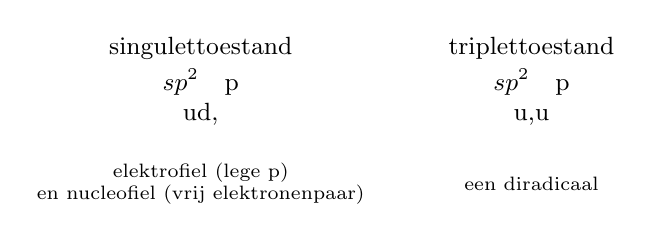
\begin{tikzpicture}[font=\small]
  \node[align=center] at (0,0) {singulettoestand\\[2pt] $sp^2$ \ \ p\\ \omorbs{ud,}};
  \node[align=center] at (4.2,0) {triplettoestand\\[2pt] $sp^2$ \ \ p\\ \omorbs{u,u}};
  \node[font=\scriptsize, align=center] at (0,-1.3) {elektrofiel (lege p)\\ en nucleofiel (vrij elektronenpaar)};
  \node[font=\scriptsize, align=center] at (4.2,-1.3) {een diradicaal};
\end{tikzpicture}

{\small Elektronenbezetting van de twee niet-bindende orbitalen van een
\omterm{def:b3:organometallic-bonding:carbene}{carbeen}. Het triplet is de grondtoestand van $\ce{CH2}$; $\pi$-donorsubstituenten (Cl, OR, $\mathrm{NR_2}$) verhogen de
orbitaal p en maken het singulet tot grondtoestand, zoals bij
dichloorcarbeen.}
\end{omfigure}

\omterm{def:b3:organometallic-bonding:carbene}{Carbenen} worden gemaakt door een diazoverbinding distikstof te laten
verliezen (door warmte, licht of een metaalkatalysator), door
$\alpha$-eliminatie (chloroform en een sterke base geven
$\ce{CCl3-}$, dat chloride verliest tot $\ce{CCl2}$), of men vermijdt ze helemaal met een
\omterm{def:b3:radicals-carbenes:carbenoid}{carbenoïde}.

\begin{definition}[Carbenoïden]\label{def:b3:radicals-carbenes:carbenoid}
Een \emph{carbenoïde}\index{carbenoide@carbenoïde} is een aan een metaal
gebonden species die een carbeengroep overdraagt zoals een vrij \omterm{def:b3:organometallic-bonding:carbene}{carbeen}
dat zou doen, zonder dat het vrije \omterm{def:b3:organometallic-bonding:carbene}{carbeen} gevormd wordt, zoals het
joodmethylzinkjodide $\ce{ICH2ZnI}$ van de reactie van Simmons-Smith.
\end{definition}

\begin{definition}[Cyclopropanering]\label{def:b3:radicals-carbenes:cyclopropanation}
\emph{Cyclopropanering}\index{cyclopropanering} is de vorming van een
cyclopropaan door additie van een \omterm{def:b3:organometallic-bonding:carbene}{carbeen} of een \omterm{def:b3:radicals-carbenes:carbenoid}{carbenoïde} aan een dubbele binding C=C.
\end{definition}

\begin{proposition}[De test van Skell]\label{prop:b3:radicals-carbenes:skell}
Een \omterm{def:b3:radicals-carbenes:carbene-states}{singuletcarbeen} addeert stereospecifiek aan een alkeen \textit{cis} of \textit{trans}, met behoud van de
relatieve configuratie; een \omterm{def:b3:radicals-carbenes:carbene-states}{tripletcarbeen} geeft beide stereo-isomeren
van het cyclopropaan.
\end{proposition}

\begin{proof}[Beargumenteerd]
Het singulet vormt beide nieuwe bindingen in één geconcerteerde stap,
zonder tijd voor rotatie. Het triplet vormt eerst één binding, wat een
1,3-diradicaal in de \omterm{def:b3:many-electron-atoms:singlet-triplet}{triplettoestand} geeft; zijn twee ongepaarde
elektronen kunnen de tweede binding pas vormen nadat een spin omklapt,
wat traag is vergeleken met de rotatie om de overgebleven enkelvoudige
binding C--C: de configuratie raakt door elkaar.
\end{proof}

\begin{omfigure}
\setchemfig{atom sep=1.8em}
\schemestart
\chemfig{H_3C-[:30]=[:0]-[:-30]CH_3}
\arrow{->[singulet $\ce{CH2}$]}[,1.6]
\chemfig{(<[:210]H_3C)-[:0](<[:330]CH_3)-[:120]-[:240]}
\schemestop
\par\medskip

{\small De test van Skell: \textit{cis}-but-2-een, met beide methylgroepen aan dezelfde kant, geeft met
een \omterm{def:b3:radicals-carbenes:carbene-states}{singuletcarbeen} alleen \textit{cis}-1,2-dimethylcyclopropaan (beide methylgroepen op wiggen,
aan hetzelfde vlak van de ring); met een \omterm{def:b3:radicals-carbenes:carbene-states}{tripletcarbeen} verschijnt ook
het isomeer \textit{trans}.}
\end{omfigure}

Singuletcarbenen voegen zich ook in in bindingen C--H. Rodium(II)carboxylaten
ontleden diazoesters tot rodiumcarbenoïden die alkenen cyclopropaneren en
zich selectief in bindingen C--H invoegen, en, met chirale liganden,
enantioselectief.

\begin{definition}[Nitrenen]\label{def:b3:radicals-carbenes:nitrene}
Een \emph{nitreen}\index{nitreen} $\mathrm{R{-}\ddot N}$ is de stikstoftegenhanger van een \omterm{def:b3:organometallic-bonding:carbene}{carbeen},
een neutraal stikstofatoom met maar zes elektronen, dat bijvoorbeeld
ontstaat door verlies van distikstof uit een azide.
\end{definition}

\section{Omleggingen naar elektronenarm koolstof}

\begin{definition}[1,2-Verschuiving]\label{def:b3:radicals-carbenes:shift}
Een \emph{1,2-verschuiving}\index{1,2-verschuiving} is de migratie van een
groep, met zijn bindend elektronenpaar, van een atoom naar het naburige
elektronenarme atoom.
\end{definition}

Bij een verschuiving van Wagner-Meerwein verhuist een alkylgroep of een
hydride naar een naburig carbokation, wat een stabieler carbokation
geeft: de carbokationomleggingen van het deel van jaar~1, nu met hun
benoemde mechanisme. Terpeenskeletten worden in de natuur hervormd door
cascades van zulke verschuivingen.

\begin{definition}[Pinacolomlegging]\label{def:b3:radicals-carbenes:pinacol}
De \emph{pinacolomlegging}\index{pinacolomlegging} zet een 1,2-diol in
zuur milieu om in een keton of een aldehyde: één hydroxygroep vertrekt
als water, een groep op het naburige koolstofatoom verschuift naar het
kation, en het gevormde kation, gestabiliseerd door het overgebleven
zuurstofatoom, verliest een proton.
\end{definition}

\begin{definition}[Migratiebereidheid]\label{def:b3:radicals-carbenes:migratory}
De \emph{migratiebereidheid}\index{migratiebereidheid} van een groep is
haar relatieve neiging om bij een \omterm{def:b3:radicals-carbenes:shift}{1,2-verschuiving} naar een elektronenarm
centrum te verhuizen.
\end{definition}

Groepen die tijdens de verschuiving goed positieve lading dragen,
migreren het best: hydride, aryl en tertiair alkyl vóór secundair,
primair en methyl. Pinacol,
$\mathrm{(CH_3)_2C(OH){-}C(OH)(CH_3)_2}$, geeft pinacolon, 3,3-dimethylbutan-2-on.

\begin{method}[Het product van een omlegging voorspellen]\label{met:b3:radicals-carbenes:rearrangement}
\begin{enumerate}
  \item Zoek het gevormde elektronenarme atoom (kation, nitreniumion,
        zuurstofatoom van een geactiveerd peroxide, \omterm{def:b3:organometallic-bonding:carbene}{carbeen} of \omterm{def:b3:radicals-carbenes:nitrene}{nitreen}) en
        de uittredende groep die het doet ontstaan.
  \item Som de groepen op het naburige atoom op die kunnen verhuizen; als
        de geometrie vastligt (oximen), kan alleen de groep anti ten
        opzichte van de uittredende groep dat.
  \item Kies anders volgens de \omterm{def:b3:radicals-carbenes:migratory}{migratiebereidheid}, of volgens welke groep
        het stabielere kation vormt op de plaats die ze verlaat.
  \item Verplaats de groep met behoud van haar configuratie, en
        vervolledig dan het mechanisme (verlies van een proton, opname van
        water).
\end{enumerate}
\end{method}

\section{Omleggingen naar elektronenarm stikstof en zuurstof}

\begin{definition}[Beckmannomlegging]\label{def:b3:radicals-carbenes:beckmann}
De \emph{beckmannomlegging}\index{beckmannomlegging} zet een oxim in
sterk zuur om in een amide: de hydroxygroep, geactiveerd als uittredende
groep, vertrekt terwijl de groep anti ten opzichte ervan van koolstof
naar stikstof migreert; water addeert aan het gevormde nitriliumion, en
tautomerisatie geeft het amide.
\end{definition}

\begin{proposition}[Anti-migratie]\label{prop:b3:radicals-carbenes:beckmann-anti}
Bij de \omterm{def:b3:radicals-carbenes:beckmann}{beckmannomlegging} migreert de groep die anti staat ten opzichte
van de uittredende groep op stikstof.
\end{proposition}

\begin{proof}[Beargumenteerd]
Het migrerende bindingspaar valt het stikstofatoom aan vanaf de
achterkant van de binding N--O, zoals bij een
verdringing $\mathrm S_\mathrm N2$; alleen de groep anti ten opzichte van het zuurstofatoom heeft zijn binding uitgelijnd met
de $\sigma^*$-orbitaal van N--O. De stap is geconcerteerd met het vertrek van de uittredende groep,
zodat er geen vrij nitreniumion ontstaat dat anders zou kunnen kiezen.
\end{proof}

\begin{omfigure}
\setchemfig{atom sep=1.9em}
\schemestart
\chemfig{*6(-----(=N-[:30]OH)-)}
\arrow{->[$\ce{H2SO4}$ (oleum)][Beckmann]}[,1.8]
\chemfig{*7(---N(-[:-90]H)-(=O)---)}
\schemestop
\par\medskip
\schemestart
\chemfig{*6(-----(=O)-)}
\arrow{->[peroxyzuur][Baeyer-Villiger]}[,1.8]
\chemfig{*7(-----O-(=O)-)}
\schemestop

{\small Twee ringvergrotingen van cyclohexanon. Boven: zijn oxim legt zich
in oleum om tot caprolactam (azepan-2-on), het monomeer van nylon-6,
waarbij stikstof in de ring komt. Onder: een peroxyzuur voegt een
zuurstofatoom in naast de carbonylgroep, wat $\varepsilon$-caprolacton (oxepan-2-on) geeft.}
\end{omfigure}

\begin{definition}[Baeyer-villigeroxidatie]\label{def:b3:radicals-carbenes:baeyer}
De \emph{baeyer-villigeroxidatie}\index{baeyer-villigeroxidatie} zet met
een peroxyzuur een keton om in een ester, of een cyclisch keton in een
lacton: het peroxyzuur addeert aan de carbonylgroep, daarna migreert een
groep op het carbonylkoolstofatoom naar het dichtstbijzijnde
peroxidezuurstofatoom terwijl een carboxylaat vertrekt.
\end{definition}

\begin{proposition}[Regiochemie van Baeyer-Villiger]\label{prop:b3:radicals-carbenes:bv-retention}
Bij de \omterm{def:b3:radicals-carbenes:baeyer}{baeyer-villigeroxidatie} behoudt de migrerende groep haar
configuratie, en de volgorde van \omterm{def:b3:radicals-carbenes:migratory}{migratiebereidheid} is tertiair alkyl >
secundair alkyl $\approx$ aryl > primair alkyl > methyl (experimenteel vastgesteld).
\end{proposition}

\begin{proof}[Beargumenteerd]
De groep verhuist met haar bindend paar over het vlak van het
koolstofatoom dat ze verlaat en komt van dezelfde kant op het
zuurstofatoom terecht, zodat haar configuratie behouden blijft. In de
overgangstoestand draagt de migrerende groep een positieve deellading,
die alkylsubstitutie en arylconjugatie stabiliseren.
\end{proof}

\begin{definition}[Isocyanaten, omleggingen van Curtius en Hofmann]\label{def:b3:radicals-carbenes:curtius}
Een \emph{isocyanaat}\index{isocyanaat} is een verbinding $\ce{R-N=C=O}$. Bij de \emph{curtiusomlegging}
\index{curtiusomlegging} verliest een acylazide bij verhitting distikstof
terwijl de groep R van koolstof naar stikstof verhuist, wat een isocyanaat
geeft; bij de \emph{hofmannomlegging}\index{hofmannomlegging} geeft een
primair amide, behandeld met broom en base, hetzelfde isocyanaat via een
N-broomamide. Met water geeft het isocyanaat het amine $\ce{RNH2}$ en koolstofdioxide; met
een alcohol een carbamaat.
\end{definition}

\begin{definition}[Ketenen en de wolffomlegging]\label{def:b3:radicals-carbenes:wolff}
Een \emph{keteen}\index{keteen} is een verbinding $\mathrm{R_2C{=}C{=}O}$. Bij de \emph{wolffomlegging}
\index{wolffomlegging} verliest een $\alpha$-diazoketon distikstof
terwijl de groep op het carbonylkoolstofatoom migreert, wat een keteen
geeft, dat water, een alcohol of een amine addeert.
\end{definition}

De \omterm{def:b3:radicals-carbenes:wolff}{wolffomlegging} is de sleutelstap van de homologering van
Arndt-Eistert, die een carbonzuur met één koolstofatoom verlengt:
zuurchloride, dan diazoketon, dan \omterm{def:b3:radicals-carbenes:wolff}{keteen}, dan het homologe zuur.

\begin{safety}{\ghs[0.62cm]{GHS06}\ghs[0.62cm]{GHS08}\ghs[0.62cm]{GHS09}}
% ledger: ghs4:Bu3SnH, ghs4:diazomethane, ghs4:AIBN
Tributyltinhydride: giftig bij inslikken, schadelijk bij contact met de
huid, beschadigt organen bij herhaalde blootstelling, zeer giftig voor in
het water levende organismen; tinresten worden gescheiden ingezameld.
Diazomethaan is een giftig, kankerverwekkend en explosief gas; het wordt
hier alleen om zijn chemie genoemd en in de praktijk vervangen door
veiligere reagentia zoals trimethylsilyldiazomethaan. AIBN is bij
verhitting zelfontledend.
\end{safety}

\begin{history}[Een radicaal dat niet zou mogen bestaan, en een nylon]
In 1900 verkreeg Moses Gomberg, die hexafenylethaan probeerde te maken,
een gele oplossing die zuurstof en jood opnam: het trifenylmethylradicaal,
het eerste persistente koolstofradicaal. Een halve eeuw later werd de
\omterm{def:b3:radicals-carbenes:beckmann}{beckmannomlegging} van cyclohexanonoxim de industriële route naar
caprolactam, dat door ringopening gepolymeriseerd wordt tot nylon-6, een
vezel en technische kunststof die op zeer grote schaal gemaakt wordt.
\end{history}

\section{Oefeningen}

\begin{exercise}[$\star$]\label{exo:b3:radicals-carbenes:1}
Bij \qty{25}{\celsius} zijn de relatieve reactiviteiten per waterstofatoom van primaire,
secundaire en tertiaire bindingen C--H $1 : 3.9 : 5.1$ tegenover chlooratomen en $1 : 82 : 1600$ tegenover
broomatomen (gegevens van de oefening). Bereken de verhoudingen van 1- en
2-halogeenpropaan die in elk geval uit propaan ontstaan.
\end{exercise}

\begin{exercise}[$\star$]\label{exo:b3:radicals-carbenes:2}
Wat is de grondtoestand van $\ce{CH2}$, en van $\ce{CCl2}$? Welk van beide addeert stereospecifiek aan
\textit{trans}-but-2-een, en wat geeft het?
\end{exercise}

\begin{exercise}[$\star$]\label{exo:b3:radicals-carbenes:3}
Geef het product van de reactie van Simmons-Smith van (\textit{Z})-hex-3-een.
\end{exercise}

\begin{exercise}[$\star$]\label{exo:b3:radicals-carbenes:4}
Geef de producten van de \omterm{def:b3:radicals-carbenes:baeyer}{baeyer-villigeroxidatie} van cyclohexanon en van
acetofenon.
\end{exercise}

\begin{exercise}[$\star\star$]\label{exo:b3:radicals-carbenes:5}
Bereken met de gegevens van \cref{exo:b3:radicals-carbenes:1} de
verhoudingen van de twee monochloriden en van de twee monobromiden van
2-methylpropaan.
\end{exercise}

\begin{exercise}[$\star\star$]\label{exo:b3:radicals-carbenes:6}
Een nieuwe \omterm{def:b3:radicals-carbenes:radical-clock}{radicaalklok}, gereduceerd met $\qty{0.020}{mol/L}$ $\mathrm{Bu_3SnH}$, geeft drie keer zoveel omgelegd
als niet-omgelegd product. Bepaal met $k_H = \qty{2.4e6}{L.mol^{-1}.s^{-1}}$ zijn snelheidsconstante.
\end{exercise}

\begin{exercise}[$\star\star$]\label{exo:b3:radicals-carbenes:7}
Deel de aanval van een hex-5-enylradicaal op C5 en op C6 in volgens de
regels van Baldwin, en zeg daarna of elk van deze sluitingen begunstigd
is: 4-exo-tet, 5-endo-trig, 5-exo-dig, 3-exo-dig, 5-endo-dig.
\end{exercise}

\begin{exercise}[$\star\star$]\label{exo:b3:radicals-carbenes:8}
Geef het product van de \omterm{def:b3:radicals-carbenes:pinacol}{pinacolomlegging} van 2,3-difenylbutaan-2,3-diol,
en verklaar de keuze van de migrerende groep.
\end{exercise}

\begin{exercise}[$\star\star$]\label{exo:b3:radicals-carbenes:9}
Benzoylazide wordt in tolueen verhit, daarna wordt water toegevoegd; in
een tweede experiment ethanol. Geef de producten.
\end{exercise}

\begin{exercise}[$\star\star\star$]\label{exo:b3:radicals-carbenes:10}
Bereken met $\mathrm{BDE(H{-}Cl)} = \qty{432}{kJ/mol}$ en $\mathrm{BDE(H{-}Br)} = \qty{366}{kJ/mol}$ (gegevens van de oefening) en de waarden C--H van
de figuur van het hoofdstuk $\Delta H$ voor de onttrekking van een primair en
van een tertiair waterstofatoom door elk halogeenatoom, en verklaar met
het postulaat van Hammond de selectiviteiten van
\cref{exo:b3:radicals-carbenes:1}.
\end{exercise}

\begin{exercise}[$\star\star\star$]\label{exo:b3:radicals-carbenes:11}
Geef de beckmannproducten van de twee oximen, \textit{E} en \textit{Z}, van 2-methylcyclohexanon,
en leg uit waarom ze verschillen, terwijl de \omterm{def:b3:radicals-carbenes:baeyer}{baeyer-villigeroxidatie} van
het keton één hoofdlacton geeft.
\end{exercise}

\begin{exercise}[$\star\star\star$]\label{exo:b3:radicals-carbenes:12}
Bereken met de modelklok van het hoofdstuk de gecycliseerde fractie bij $[\mathrm{Bu_3SnH}] = 0.010$,
0.10 en \qty{1.0}{mol/L}. Welke hydrideconcentratie geeft 95\,\% gecycliseerd product, en hoe
kan men die aanhouden?
\end{exercise}

\section{Probleem: twee ringen uit cyclohexanon}

\begin{problem}[{Weekendprobleem --- twee ringen uit cyclohexanon: het
oxim, de beckmannomlegging tot caprolactam, de baeyer-villigeroxidatie
tot caprolacton, en de regiochemie van beide met 2-methylcyclohexanon}]
\label{pb:b3:radicals-carbenes:1}
% ledger: aw:C, aw:H, aw:N, aw:O, aw:S
Gegevens van het probleem: één ton cyclohexanon wordt met een rendement
van 98\,\% omgezet in zijn oxim, en het oxim met een rendement van
98\,\% in caprolactam; de omlegging gebruikt
1.3 mol zwavelzuur (als oleum) per mol oxim, dat op het einde met
ammoniak geneutraliseerd wordt tot ammoniumsulfaat.

\medskip\noindent\textbf{Deel I --- Het oxim.}
\begin{enumerate}
  \item Schrijf de vorming van cyclohexanonoxim uit hydroxylamine op.
  \item Waarom werkt men rond pH 4 à 5?
  \item Heeft cyclohexanonoxim isomeren \textit{E} en \textit{Z}? Waarom?
  \item Teken de oximen \textit{E} en \textit{Z} van 2-methylcyclohexanon.
  \item Waarom gaan deze twee oximen maar traag in elkaar over?
\end{enumerate}

\medskip\noindent\textbf{Deel II --- De \omterm{def:b3:radicals-carbenes:beckmann}{beckmannomlegging}.}
\begin{enumerate}[resume]
  \item Wat doet het zuur met het oxim?
  \item Welke binding migreert, en waarom maakt dat de ring groter?
  \item Welk intermediair valt water aan?
  \item Schrijf de totaalvergelijking op, van oxim tot caprolactam.
  \item Benoem en teken het product, en het polymeer dat ervan gemaakt
        wordt.
  \item Bereken de molaire massa's van cyclohexanon en caprolactam.
  \item Bereken de massa caprolactam uit één ton cyclohexanon.
  \item Bereken de massa ammoniumsulfaat die daarbij ontstaat.
\end{enumerate}

\medskip\noindent\textbf{Deel III --- De \omterm{def:b3:radicals-carbenes:baeyer}{baeyer-villigeroxidatie}.}
\begin{enumerate}[resume]
  \item Schrijf de oxidatie van cyclohexanon door een peroxyzuur $\ce{RCO3H}$ op.
  \item Geef het intermediair dat ontstaat door additie van het
        peroxyzuur.
  \item Welke groep migreert, en wat is de uittredende groep?
  \item Benoem het lacton en het polymeer dat het geeft.
  \item Waarom kan waterstofperoxide met een katalysator het peroxyzuur
        vervangen in een schoner proces?
\end{enumerate}

\medskip\noindent\textbf{Deel IV --- 2-Methylcyclohexanon.}
\begin{enumerate}[resume]
  \item Welk koolstofatoom migreert bij zijn \omterm{def:b3:radicals-carbenes:baeyer}{baeyer-villigeroxidatie}, en
        welk lacton ontstaat?
  \item Blijft de configuratie van dat koolstofatoom behouden?
  \item Welk lactam geeft het oxim \textit{E} (OH anti ten opzichte van het koolstofatoom met de methylgroep)?
  \item Welk lactam geeft het oxim \textit{Z}?
  \item Wat bepaalt de regiochemie in elke reactie?
  \item Waarom heeft cyclohexanon zelf deze problemen niet?
  \item Formuleer het resultaat: de massa caprolactam uit één ton
        cyclohexanon.
\end{enumerate}
\end{problem}
